% 图 3.9 NMR 装置示意：电磁铁两极产生 B0，样品置于 RF 线圈中，B1 垂直于 B0
\documentclass[tikz,border=5pt]{standalone}
\usetikzlibrary{arrows.meta,patterns}
\usepackage{amsmath}
\usepackage{bm}
\usepackage{fontspec}
\setmainfont{Times New Roman}
\begin{document}
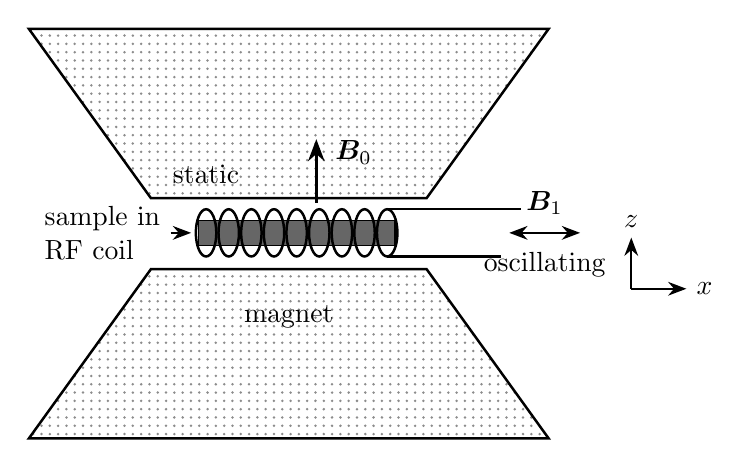
\begin{tikzpicture}[line width=0.8pt,>=Stealth]
% 上磁极（梯形剖面，点纹填充）
\filldraw[fill=white,pattern=dots,pattern color=black!45,line width=0.9]
  (-3.30,4.35) -- (3.30,4.35) -- (1.75,2.20) -- (-1.75,2.20) -- cycle;
% 下磁极
\filldraw[fill=white,pattern=dots,pattern color=black!45,line width=0.9]
  (-1.75,1.30) -- (1.75,1.30) -- (3.30,-0.85) -- (-3.30,-0.85) -- cycle;
% 样品（灰色长条）
\filldraw[fill=black!60,line width=0.5] (-1.15,1.60) rectangle (1.35,1.92);
% RF 线圈（约 10 匝）
\foreach \x in {-1.05,-0.7625,...,1.30}{
  \draw[line width=0.9] (\x,1.76) ellipse [x radius=0.13,y radius=0.30];
}
% 引线（右侧两根）
\draw[line width=0.8] (1.25,2.06) -- (2.95,2.06);
\draw[line width=0.8] (1.25,1.46) -- (2.70,1.46);
% 标注：static / B0
\node at (-1.05,2.50) {static};
\draw[->,line width=1.1] (0.35,2.14) -- (0.35,2.95);
\node[anchor=west] at (0.46,2.78) {$\boldsymbol{B}_0$};
% 标注：magnet
\node at (0,0.70) {magnet};
% 左侧样品标签
\node[anchor=east,align=left,inner sep=2pt] at (-1.55,1.76) {sample in\\RF coil};
\draw[->] (-1.50,1.76) -- (-1.24,1.76);
% 右侧 B1 振荡场
\draw[<->,line width=0.8] (2.80,1.76) -- (3.70,1.76);
\node[anchor=south] at (3.25,1.86) {$\boldsymbol{B}_1$};
\node[anchor=north] at (3.25,1.64) {oscillating};
% 右上坐标系（B0//z, B1//x）
\draw[->] (4.35,1.05) -- (4.35,1.70) node[above]{$z$};
\draw[->] (4.35,1.05) -- (5.05,1.05) node[right]{$x$};
\end{tikzpicture}
\end{document}
